\section{Strömungslinien}
\label{joukowski:sec:stroemungslinien}
\kopfrechts{Strömungslinien}
	\subsection{Allgemeine Definition}
		Die Bewegung von Fluiden im dreidimensionalen Raum wird durch die Navier-Stokes-Gleichungen
		oder die reibungsfreien Euler-Gleichungen beschrieben.
		Dabei handelt es sich um komplizierte partielle Differentialgleichungen,
		deren Anwendung für dieses Seminar zu weit führt.
		Hier geht es nur darum, den physikalischen Ursprung mit den komplexen Zahlen in Verbindung zu bringen.
		Das exakte Verständnis für die Entstehung der Strömungsgleichung wird nicht vorausgesetzt.
		
		Haben wir eine inkompressible Strömung in zwei Dimensionen,
		können wir aus der Bedingung~\eqref{joukowski:voraussetzungen:inkompressibel} schliessen,
		dass eine sogenannten Potentialfunktion $\varphi$ existiert,
		welche sich mit
		\[
			\vec{v}
			=
			\nabla \varphi.
		\]
		berechnen lässt.
		Dies beschreibt die Situation einer sogenannter \emph{Potentialströmung}.
\index{Potentialstromung@Potentialströmung}%
		Setzen wir unsere Gleichung für $\varphi$ in die Bedinung der Inkompressibilität des Fluides aus Gleichung~\eqref{joukowski:voraussetzungen:inkompressibel} ein,
		erhalten wir die Laplace-Gleichung
\index{Laplace-Gleichung}%
		\[
			\nabla \cdot \nabla \varphi
			=
			\Delta \varphi
			=
			0.
		\]
		Das beduetet jede Potentialfunktion, welche die Strömung eines inkompressiblen, laminaren Fluid beschreibt, muss die Laplace-Gleichung erfüllen.
\index{Potentialfunktion}%
		Aus Abschnitt~\ref{joukowski:voraussetzungen:situationsbeschreibung}
		wissen wir aber, dass das Problem auf zwei Dimensionen begrenzt werden kann.
		Sobald die Strömung nur von $x$ und $y$ abhängig ist,
		können wir die komplexen Zahlen zur Hand nehmen und die Situation vereinfacht sich wesentlich.
		Wir formulieren eine komplexe Funktion $f(z)$, welche die Strömung unseres Fluides mit der Gleichung
		\[
			f(z)
			= 
			\varphi(z) + i \psi(z)
		\]
		beschreibt, wobei $\varphi(z)$ unserer oben erwähnten Potentialfunktion entspricht.
		Dabei können wir ausnutzen, dass der Realteil einer holomorphen Funktion automatisch die Laplace-Gleichung erfüllt.
		Wir können daraus nun den folgenden Satz formulieren.
		
		\begin{satz}
			Jede holomorphe Funktion $f(z)$ erfüllt die Laplace-Gleichung
			und ist eine gültige Beschreibung einer Fluidströmung in zwei Dimensionen.
			\label{joukowski:stroemungslinien:satz:holomorphe-funktion}
		\end{satz}
		
		Jetzt können wir alle Werkzeuge der komplexen Analysis anwenden, um unsere Strömung zu beschreiben.		
		Punkte in der $z$-Ebene, für welche die Potentialfunktion $\varphi(z)$ den gleichen Wert hat, werden \emph{Äquipotentiallinien} genannt
		und Punkte, für welche $\psi(z)$ konstant ist, werden \emph{Strömungslinien} genannt.
\index{Aquipotentiallinien@Äquipotentiallinien}%
		Für unsere weiteren Betrachtungen sind die Strömungslinien von grosser Bedeutung.
		
		\begin{definition}[Strömungslinie]
			\label{joukowski:stroemungslinien:proof:Stroemungslinie}
			In der stationären Strömung beschreibt eine \emph{Strömungsline} den Weg, welcher ein Fluidteilchen nimmt
\index{Stromungslinie@Strömungslinie}%
			und gilt für alle Punkte $z$ die
			\[
				\psi(z) = C
			\]
			erfüllen.
		\end{definition}
		Unterschiedliche Konstanten $C$ bezeichnen dabei unterschiedliche Strömungslinien.
		Um diese übersichtlich darzustellen, beschränken wir uns bei der Visualisierung auf eine diskrete Anzahl Konstanten $C$ aus der Definition~\ref{joukowski:stroemungslinien:proof:Stroemungslinie}.
		
		\begin{figure}
	\centering
	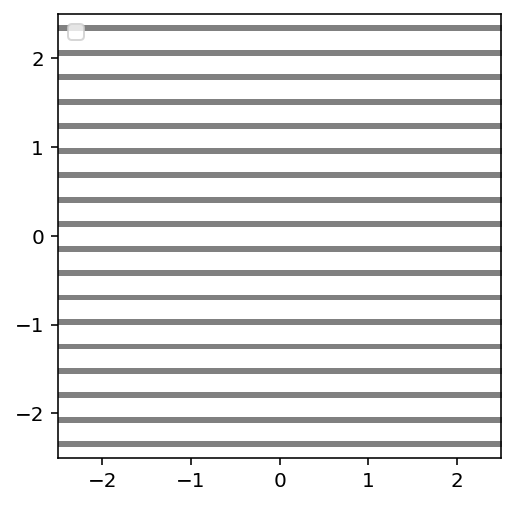
\includegraphics[width=0.45\textwidth]{papers/joukowski/images/05_stroemungslinien/Strom_g.png}
	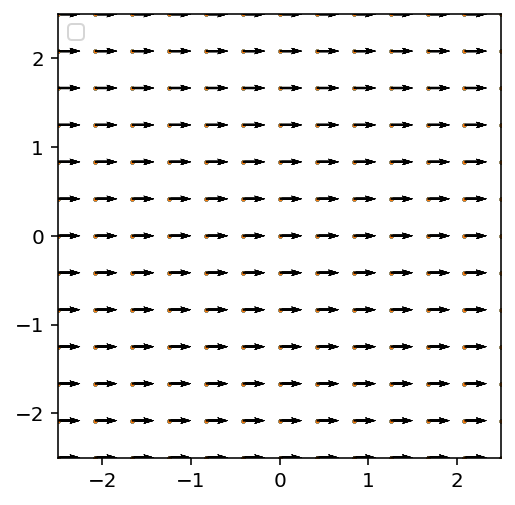
\includegraphics[width = 0.45\textwidth]{papers/joukowski/images/05_stroemungslinien/speed.png}
\end{figure}

		\begin{beispiel}
			\label{joukowski:stroemungslinien:beispiel:ungestoerte-Stroemung}
			Beginnen wir mit einer möglichst einfachen Strömung: Eine homogene, ungehinderte Strömung von links nach rechts, wie in Abbildung~\ref{joukowski:Stroemungslinien:fig_Allgemein}.
			Es wird sofort deutlich, dass die Strömungslinien horizontal verlaufen und vertikal gleichmässig verteilt sind.
			Somit ist die Geschwindigkeit an jedem Punkt des Raumes identisch.
		%	Die Abbildung~\ref{joukowski:Stroemungslinien:fig_Allgemein}, welche dieser Situation entspricht,
Diese Situation
			kann mit der holomorphen Strömungsfunktion $f(z) = z$ und der konstanten Geschwindigkeitsfunktion ${v(z)} = 1$ beschrieben werden.
		\end{beispiel}
		
		\begin{figure}
	\centering
	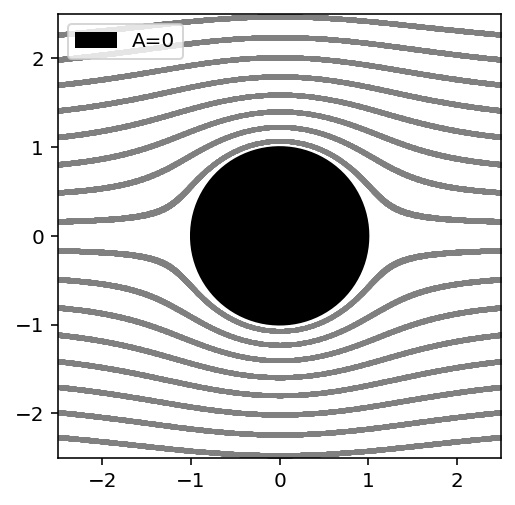
\includegraphics[width=0.45\textwidth]{papers/joukowski/images/05_stroemungslinien/Magnus_Strom_A000_g.png}
	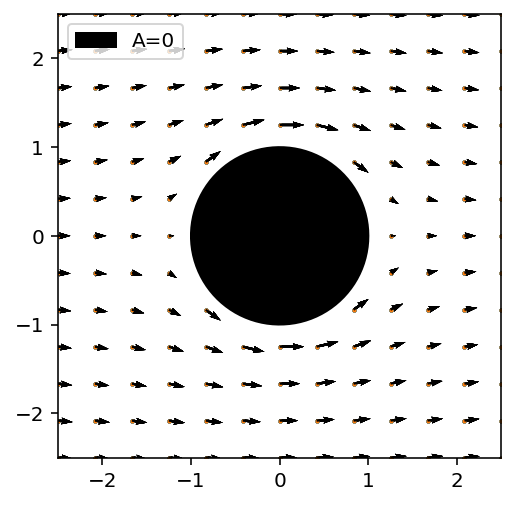
\includegraphics[width = 0.45\textwidth]{papers/joukowski/images/05_stroemungslinien/Magnus_Speed_A000.png}
\end{figure}

		\begin{beispiel}
		\label{joukowski:stroemungslinien:beispiel:joukowski-transformation}
		Wir fügen einen Zylinder als Hindernis ein.
		Im unserer zweidimensionalen Betrachtung gilt dieser Zylinder als Kreis mit Schwerpunkt im Ursprung, wie in Abbildung~\ref{joukowski:Stroemungslinien:fig_Zylinder} dargestellt.
		Um diese Situation zu analysieren, müssen wir eine komplexe Funktion finden,
		welche unser Hindernis auf eine horizontale Linie abbildet.
		Eine eine horizontale Linie als ``Hindernis'' entspricht der gleichen Situation wie in Beispiel~\ref{joukowski:stroemungslinien:beispiel:ungestoerte-Stroemung}.
		Finden wir diese Funktion,
		so bildet diese auch die Strömungslinien um das Hindernis auf die horizontalen Strömungslinien aus Beispiel~\ref{joukowski:stroemungslinien:beispiel:ungestoerte-Stroemung} ab.
		Diese Eigenschaft gilt nur,
		wenn diese Funktion \emph{biholomorph} ist.
		
		\begin{definition}[Biholomorphe Funktion]
			Eine komplexe Funktion $f(z)$ ist \emph{biholomorph}, wenn
\index{biholomorph}%
			\begin{enumerate}
				\item $f(z)$ holomorph ist
				und
				\item ihre Umkehrfunktion $f^{-1}(z)$ auch holomorph ist.
			\end{enumerate}
		\end{definition}
		
		Die komplexe Funktion, welche einen Kreis im Ursprung auf eine horizontale Linie abbildet, ist die sogenannte \emph{Kutta-Joukowski-Transformation} und lautet
\index{Kutta-Joukowski-Transformation}%
		\begin{equation}
			\label{joukowski:Stroemungslinien:equation_zylinder}
			f(z)
			=
			v_\infty \cdot \biggl(z+\frac{1}{z}\biggr).
		\end{equation}
		Die Ableitung dieser Funktion nach $z$ ist dann
		\begin{equation}
			\label{joukowski:Stroemungslinien:equation_zylinder_speed}
			\frac{df}{dz}
			=
			\overline{v(z)}
			=
			v_\infty \cdot \biggl(1 - \frac{1}{z^2}\biggr).
		\end{equation} 
		Die Strömungslinien dieser Funktion sowie die Geschwindigkeiten werden in Abbildung ~\ref{joukowski:Stroemungslinien:fig_Zylinder} dargestellt.
		\end{beispiel}
		
	\subsection{Zusammenhang zwischen $f(z)$ und $\overline{v(z)}$}
		\label{joukowski:stroemungslinien:zusammenhang-fz-z}
		In Beispiel~\ref{joukowski:stroemungslinien:beispiel:joukowski-transformation}
		haben wir
		\begin{equation}
			\label{joukowski:stroemungslinien:dfdz}
			\frac{df}{dz}
			=
			\overline{v(z)}
		\end{equation}
geschrieben.
		Dies scheint auf den ersten Blick etwas merkwürdig zu sein,
		da im Reellen die Ableitung direkt die Geschwindigkeit selbst gibt.
		Dieses Resultat stammt aus den Cauchy-Riemann-Differentialgleichungen und der Konvention \eqref{joukowski:vkonvention},
\index{Cauchy-Riemann-Differentialgleichungen}%
		die komplexe Geschwindigkeit als $v(z) = u + iw$ zu schreiben.
		
		\begin{proof}[Beweis von Formel~\eqref{joukowski:stroemungslinien:dfdz}]
			\label{joukowski:stroemungslinien:v-konjugiert-komplex}
			Wir berechnen die komplexe Ableitung der Funktion $f(z)$ nach $z$.
			Als erstes teilen wir $f(z)$ in Real- und Imaginärteil auf und schreiben
			\[
				\frac{df}{dz}
				=
				\frac{d\varphi}{dz} + i \frac{d\psi}{dz}.
			\]
			Jetzt können wir ausnutzen, dass es bei einer holomorphen Funktion keine Rolle spielt, in welche Richtung die Ableitung erfolgt,
			was heisst, dass
			\[
				\frac{df}{dz}
				=
				\frac{\partial f}{\partial x}
				=
				\frac{1}{i} \cdot \frac{\partial f}{\partial y}
			\]
			gilt.
			Dabei nutzen wir aus den Cauchy-Riemann-Differentialgleichungen die Zusammenhänge
			\[
				\frac{d\varphi}{dz}
				=
				\frac{\partial \varphi}{\partial x}
				\qquad
				\text{und}
				\qquad
				\frac{d\psi}{dz}
				=
				-\frac{\partial \varphi}{\partial y}.
			\]
Nach der Konvention \eqref{joukowski:vkonvention} für die Komponenten
der Geschwindigkeit bietet sich an,
			%Es ist üblich,
			\[
				u
				=
				\frac{\partial \varphi}{\partial x}
				\qquad
				\text{und}
				\qquad
				w
				=
				\frac{\partial \varphi}{\partial y}
			\]
			zu schreiben.
			Somit ergibt sich schliesslich
			\[
				\frac{df}{dz}
				=
				u - iw
				=
				\overline{v(z)}. \qedhere
			\]
		\end{proof}
	
